%-----------------------------------------------------------------------
%
%   UFRJ  - Universidade Federal do Rio de Janeiro
%   COPPE - Coordena��o dos Programas de P�s-gradua��o em Engenharia
%   PEE   - Programa de Engenharia El�trica
%
%   COE-835  Controle adaptativo
%
%   Relat�rio da simula��o
%                                                         Ramon R. Costa
%                                                         05/out/09, Rio
%-----------------------------------------------------------------------
\documentclass[11pt,a4paper]{article}
\usepackage[latin1]{inputenc} %pacote para utilizar palavras acentuadas
\usepackage{amsmath,amssymb}  %pacotes do AMS
\usepackage{latexsym}         %pacote para incluir s�mbolos (ex.\Box)
\usepackage{fancybox,fancyhdr}%pacote com frescuras
\usepackage{graphicx}         %pacote para incluir figuras tipo eps
\usepackage[portuguese]{babel}
\usepackage{xcolor}
\usepackage{float} 
\usepackage{epstopdf}
\usepackage[inline]{enumitem}
\usepackage[a4paper]{hyperref}% Make sure it comes last of your loaded packages
\hypersetup{
  verbose,
  plainpages=false,
  bookmarks=true,
  colorlinks=true,
  linkcolor=blue
}
     
%----------------------------------------------------------------------
%
%   Macros utilizados no LATEX
%                                                       Ramon R. Costa
%                                                       13/out/17, Rio
%----------------------------------------------------------------------
\newcount\m
\newcount\n

\def\twodigits#1{\ifnum #1<10 0\fi \number#1}

\def\hours{\n=\time \divide\n 60
    \m=-\n \multiply\m 60 \advance\m \time
    \twodigits\n:\twodigits\m}

\def\hora{\hours}

\def\fim{
  \medskip
  \begin{center}
    \rule[1mm]{30mm}{0.14mm}$\diamond$\rule[1mm]{30mm}{0.14mm}
  \end{center}
}

%----------------------------------------------------------------------
% A4 paper size & margins
\setlength {\textheight}    {25cm}%
\setlength {\textwidth}     {17.5cm}%
\setlength {\parindent}     {0mm}%
\setlength {\parskip}       {1mm}%
\setlength {\topmargin}     {-14mm}%
\setlength {\oddsidemargin} {-6mm}%
\setlength {\evensidemargin}{-6mm}%
\setlength {\columnsep}     {6mm}%

%----------------------------------------------------------------------
\def\codigo{COE-835}
\def\disciplina{Controle adaptativo}
\def\periodo{3o. período/2017}
\def\professor{Ramon}

\newcommand{\BOX}[1]{
  \framebox{{\color{magenta}\rule[-3mm]{1mm}{9mm}} ~~$\displaystyle
  \begin{aligned} #1 \end{aligned}$~~}\pagestyle{plain}
}

\newcommand{\RED}[1]{\colorbox{white}{\textcolor{red}{#1}}}
%\newcommand{\WoR}[1]{\colorbox{red}{\textcolor{white}{#1}}}
\newcommand{\BLU}[1]{\colorbox{white}{\textcolor{blue}{#1}}}
\newcommand{\GRE}[1]{\colorbox{green}{\textcolor{black}{#1}}}
\newcommand{\HI}[1]{\colorbox{yellow}{\textcolor{black}{#1}}}  %% Highlithed text

\newcommand{\estrela}[1]{
  \def\TXT{\RED{$\bigstar$ }}
  \hspace*{5mm}\TXT \hfill
  \parbox[t]{ \textwidth - \widthof{\TXT} - 5mm}{#1}
  \par
}

\def\Ltwo{\mbox{${\mathcal L}_2$}}
\def\Linf{\mbox{${\mathcal L}_\infty$}}

\newcommand{\sign}{\mbox{sign}}

\newcommand{\equacao}[2]{
  \makebox[40mm][l]{#1 \dotfill}: \quad \parbox[t]{8cm}
	{\begin{equation} \displaystyle
  \begin{aligned}
    #2
  \end{aligned} \end{equation}} \\
}

\newcommand{\sref}[1]{Section~\ref{#1}}
\newcommand{\fref}[1]{Fig.~\ref{#1}}
\newcommand{\tref}[1]{Table~\ref{#1}}
\newcommand{\thref}[1]{Theorem~\ref{#1}}
\newcommand{\aref}[1]{Assumption~\ref{#1}}
\newcommand{\norm}[1]{\left\lVert#1\right\rVert}
%\renewcommand{\qedsymbol}{}
\newcommand{\rev}[1]{{\color{red}#1}}
%\newcommand{\mat}[1]{\begin{bmatrix}#1\end{bmatrix}}

\newtheorem{remark}{Remark}
\newtheorem{lemma}{Lema}

\newcommand{\mat}[1]{\begin{bmatrix}#1\end{bmatrix}}

%----------------------------------------------------------------------


%Set normal paragraph spacing
\setlength\parindent{24pt}

\begin{document}
%---------------------------------------------------------------------
\pagestyle{fancy}%
\renewcommand{\headrulewidth}  {0.4pt}%
\renewcommand{\footrulewidth}  {0.4pt}%
\lhead{\bfseries{Relat�rio do Trabalho 3}}%
\chead{}%
\rhead{\bfseries\thepage}%
\lfoot{}%
\cfoot{}%
\rfoot{[\hours] \quad \today}%
%---------------------------------------------------------------------
\begin{center}
  \huge{COE-835  Controle  adaptativo}  \\[20mm]

  \Large{Trabalho 4} \\[20mm]
\end{center}

\textbf{Grupo:} \quad \parbox[t]{10cm}{
Guilherme Pires Sales de Carvalho \\[2mm]
Matheus Ferreira dos Reis \\[2mm]
Renan Salles de Freitas \\[10mm]
}

\textbf{Algoritmo:} \quad \HI{C�lculo de Par�metros para Controle 2DOF}\\[2mm]

%---------------------------------------------------------------------
\tableofcontents
\newpage
%---------------------------------------------------------------------
%---------------------------------------------------------------------
\section{Resumo do Problema}

Neste trabalho, vamos abordar o c�lculo dos par�metros ideais ${\theta^*}^T = \mat{{\theta_1^*}^T & \theta_n^* & {\theta_2^*}^T & {\theta_{2n}^*}^T}$ e o polin�mio $\Lambda(s)$ do filtro $\frac{1}{\Lambda(s)}$ utilizados em uma estrutura de dois graus de liberdade (\textit{feedback} + \textit{feedforward}). O objetivo dessa estrutura de controle � fazer com que uma planta \textbf{conhecida} $P(s) = K_p \frac{N(s)}{D(s)}$ se comporte como um modelo de refer�ncia $P_m(s) = K_m\frac{N_m(s)}{D_m(s)}$ em regime. A fun��o que calcula esses par�metros deve ser geral e resolver o problema para qualquer planta de ordem $n$ e grau relativo $n^*$.

A estrat�gia utilizada � filtrar os sinais dispon�veis no sistema (entrada e sa�da da planta) e usar combina��es lineares dos estados dos dois filtros atrav�s dos par�metros $\theta^*$ a serem encontrados. Esses sinais s�o somados ao sinal de entrada $r$ multiplicado por um ganho $\theta^*_{2n}$ tamb�m a ser encontrado.
%
O diagrama de blocos da implementa��o de controle 2DOF pode ser visto na \fref{fig:blocks} e sua forma em estrutura 2DOF � mostrada na figura \fref{fig:blocks_2DOF}.
%
\begin{figure}[H]
  \centering
  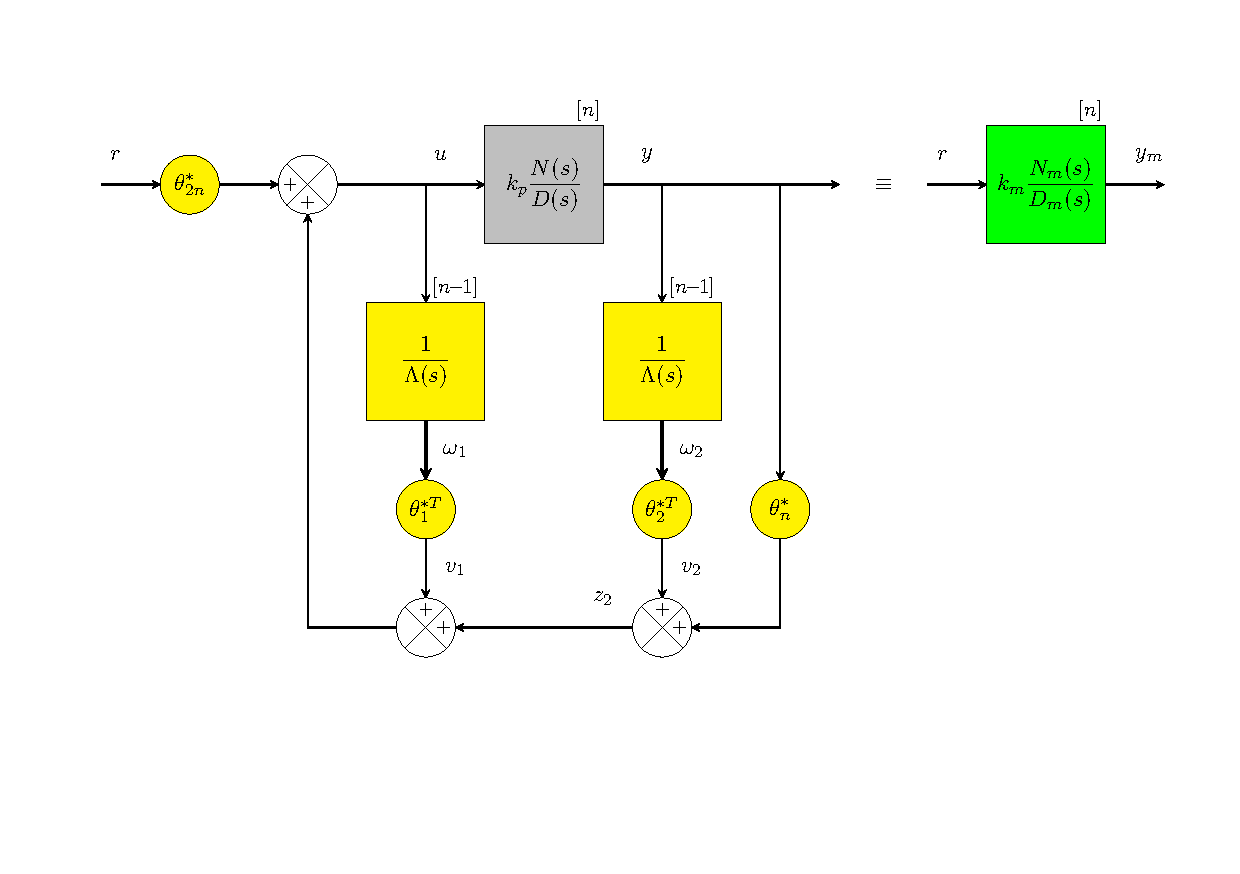
\includegraphics[width=\columnwidth]{figs/blocks.pdf}
  \caption{Implementa��o da estrutura de controle 2DOF geral.}
  \label{fig:blocks}
\end{figure}
%
\begin{figure}[H]
  \centering
  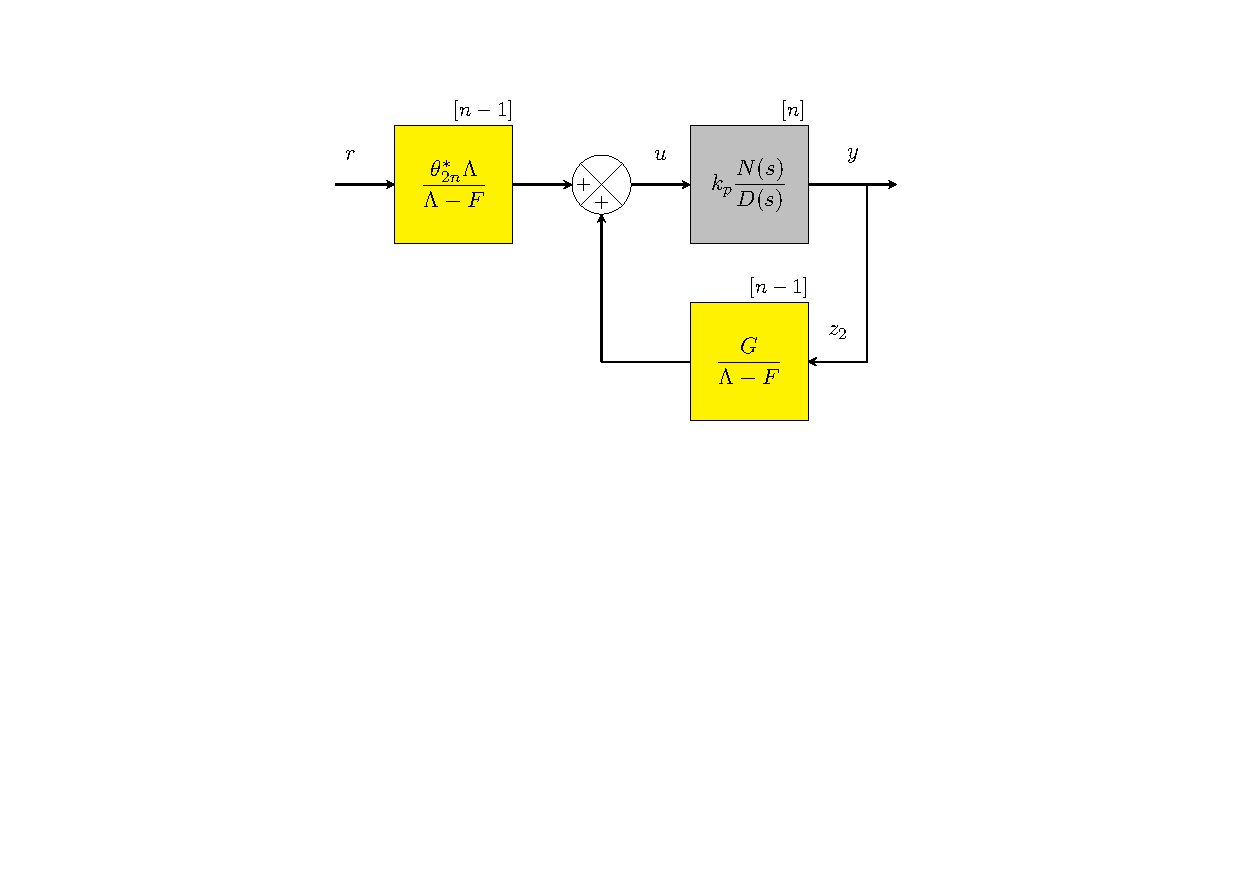
\includegraphics[width=.5\columnwidth]{figs/blocks_2DOF.pdf}
  \caption{Estrutura de controle 2DOF geral.}
  \label{fig:blocks}
\end{figure}

Nessa estrutura, temos um filtro $\frac{1}{\Lambda(s)}$ atuando sobre a entrada de controle $u$ com:
%
\begin{equation}
\Lambda(s) = s^{n-1} + \lambda_{n-2} \, s^{n-2} + \ldots + \lambda_{1} \, s + \lambda_0 \,, \qquad \text{grau}(\Lambda) = n-1 \,.
\end{equation}

A din�mica entre a sa�da $v_1$ e a entrada $u$ do filtro � dada pela equa��o de estados:
%
\begin{equation}
\textrm{Filtro 1: \quad}
\left\{ \begin{array}{l}
         \dot{\omega}_1 = A_f \, \omega_1 + b_f \, u \\
         v_1 = {\theta_1^*}^T \omega_1
        \end{array}
 \right.
 \quad \Rightarrow \quad
 v_1 = \frac{F}{\Lambda} \, u \,,
\end{equation}
%
em que utilizamos a forma can�nica control�vel para a escolha da matriz $A_f$ e do vetor $b_f$:
%
\begin{equation}
 A_f = \mat{
 0 & 1 & 0 & \cdots & 0 & 0 \\
 0 & 0 & 1 & \cdots & 0 & 0 \\
 \vdots & \vdots & \vdots & \ddots & \vdots & \vdots \\
 0 & 0 & 0 & \cdots & 1 & 0 \\
 0 & 0 & 0 & \cdots & 0 & 1 \\
 -\lambda_{0} & -\lambda_{1} & -\lambda_{2} & \cdots & -\lambda_{n-3} & -\lambda_{n-2} \\
 } \in \mathbb{R}^{(n-1) \times (n-1)} \,,
 %
 \qquad
 %
 b_f = \mat{0 \\ 0 \\ \vdots \\ 0 \\ 0 \\ 1} \in \mathbb{R}^{n-1}
\end{equation}

Resolvendo a equa��o de estados para encontrar a fun��o de transfer�ncia entre $v_1$ e $u$ atrav�s de $\frac{F}{\Lambda} = {\theta_1^*}^T \left(sI - A_f \right)^{-1} b_f$, obt�m-se:
%
\begin{align}
 F(s) &= f_{n-2} \, s^{n-2} + f_{n-3} \, s^{n-3} + \ldots + f_{1} \, s + f_0 \,, \qquad\qquad \text{grau}(F) = n-2 \nonumber \\
 &= {\theta_1^*}^T \, \mat{1 & s & s^2 & \cdots & s^{n-3} & s^{n-2}}^T \,,
\end{align}
%
de onde obt�m-se que ${\theta_1^*}^T \in \mathbb{R}^{n-1}$ s�o os coeficientes do polin�mio $F(s)$.

J� o segundo filtro recebe como entrada a sa�da da planta $y$ e cont�m um termo direto, com a seguinte implementa��o em espa�o de estados:
%
\begin{equation}
\textrm{Filtro 2: \quad}
\left\{ \begin{array}{l}
         \dot{\omega}_2 = A_f \, \omega_2 + b_f \, u \\
         z_2 = {\theta_2^*}^T \omega_2 + \theta_n^* \, y
        \end{array}
 \right.
 \quad \Rightarrow \quad
 z_2 = \frac{G}{\Lambda} \, y \,,
\end{equation}

Resolvendo a equa��o de estados para encontrar a fun��o de transfer�ncia entre $z_2$ e $y$ atrav�s de $\frac{G}{\Lambda} = {\theta_2^*}^T \left(sI - A_f \right)^{-1} b_f + \theta_n^*$, obt�m-se:
%
\begin{align}
 G(s) &= g_{n-1} \, s^{n-1} + g_{n-2} \, s^{n-2} + \ldots + g_{1} \, s + g_0 \,,\qquad\qquad \text{grau}(G) = n-1 \nonumber \\
 &= {\theta_2^*}^T \, \mat{1 & s & s^2 & \cdots & s^{n-3} & s^{n-2}}^T + \Lambda(s) \, \theta_n^* \,,
 \label{eq:theta2}
\end{align}

Sendo ${\theta_2^*}^T = \mat{\theta^*_{2_{(n-1)}} & \theta^*_{2_{(n-2)}} & \cdots & \theta^*_{2_{(2)}} & \theta^*_{2_{(1)}}}$ e tomando somente os coeficientes dos polin�mios de \eqref{eq:theta2} em ambos os lados em forma de vetor, temos:
%
\begin{equation}
 \mat{g_{n-1} & g_{n-2} & \cdots & g_1 & g_0} = \mat{\theta_n^* & \left( \theta^*_{2_{(n-1)}} + \theta_n^* \, \lambda_{n-2} \right) & \cdots & \left( \theta^*_{2_{(2)}} + \theta_n^* \, \lambda_{1} \right) & \left( \theta^*_{2_{(1)}} + \theta_n^* \, \lambda_{0} \right)} \,.
\end{equation}
%
de onde � poss�vel obter os valores de $\theta_n^*$ e $\theta_2^*$:
%
\begin{align}
 \theta_n^* &= g_{n-1} \\
 \theta_2^* &= G(2:\text{end}) - \theta_n^* \, \Lambda(2:\text{end})
\end{align}


\section{Implementa��o}

A implementa��o foi desenvolvida em MATLAB, de forma num�rica. Foi constru�da uma fun��o que recebe a fun��o de transfer�ncia da planta $P(s) = k_p \frac{N}{D}$, a fun��o de transfer�ncia do modelo $P_m(s) = k_m \frac{N_m}{D_m}$ e o polin�mio do observador $A_0$.
%
A fun��o \textit{find2DOFparameters} retorna os par�metros ideais ${\theta^*}^T = \mat{{\theta_1^*}^T & \theta_n^* & {\theta_2^*}^T & {\theta_{2n}^*}^T}$ e o polin�mio $\Lambda(s)$ do filtro para fins de implementa��o. Seu c�digo � apresentado abaixo:

\lstinputlisting[style=myMatlab]{../matlab/find2DOFparameters.m}
%[style=myMatlab,escapechar=!,float=htb]
%%---------------------------------------------------------------------
\section{Resultados}

Avaliamos o funcionamento da fun��o que calcula os par�metros ideais de controle 2DOF plantas de ordens e graus relativos distintos, assim como diferentes polin�mios $A_0$ para o observador. 
%
Abaixo, fornecemos quatro exemplos para plantas de grau relativo $n^{*} = 1, 2, 3$ e $n^{*} = 4$. Para todas as plantas consideradas, obtivemos exatamente a mesma fun��o de transfer�ncia escolhida inicialmente como modelo de refer�ncia, o que mostra a corretude do algoritmo.

%---------------------------------------------------------------------
\subsection{Simula��o \#1 ($n = 2, n^{*} = 1, n_p = 4$)}

\begin{align*}
  P(s) &= \frac{2\left(s+1\right)}{s^2 -2s + 1}\,,  &  P_m(s) &= \frac{s+2}{s^2 + 4s + 1}\,, & A_0(s) &= 1
\end{align*}

Script de teste \textit{parameters\_214}:
%
\lstinputlisting[style=myMatlab]{../matlab/parameters_214.m}

A fun��o \textit{find2DOFparameters} retornou os seguintes valores:
%
\begin{align*}
 \theta_1^* = 1 \,, \qquad \theta_n^* = -3 \,, \qquad \theta_2^* = 6 \,, \qquad \theta_{2n}^* = 0.5 \qquad \Lambda(s) = s + 2
\end{align*}

%
A sa�da da fun��o \textit{calculate2DOFmodelTF} comprovou que esses valores encontrados resultam em $Y(s)/R(s) = P_m(s)$, igual ao modelo de refer�ncia proposto, dada a planta $P(s)$.
%

%---------------------------------------------------------------------
\subsection{Simula��o \#2 ($n = 3, n^{*} = 2, n_p = 5$)}

\begin{align*}
  P(s) &= \frac{2\left(s+1\right)}{s^3 +s^2 -2s + 1}\,,  &  P_m(s) &= \frac{1}{s^2 + 4s + 1}\,, & A_0(s) &= s+1
\end{align*}

Script de teste \textit{parameters\_325}:
%
\lstinputlisting[style=myMatlab]{../matlab/parameters_325.m}

A fun��o \textit{find2DOFparameters} retornou os seguintes valores:
%
\begin{align*}
 {\theta_1^*}^T = \mat{-4 & -4} \,, \qquad \theta_n^* = -3.5 \,, \qquad {\theta_2^*}^T = \mat{-0.5 & 5.5} \,, \qquad \theta_{2n}^* = 0.5 \qquad \Lambda(s) = s^2 + 2s + 1
\end{align*}

%
A sa�da da fun��o \textit{calculate2DOFmodelTF} comprovou que esses valores encontrados resultam em $Y(s)/R(s) = P_m(s)$, igual ao modelo de refer�ncia proposto, dada a planta $P(s)$.

%---------------------------------------------------------------------
\subsection{Simula��o \#3 ($n = 3, n^{*} = 3, n_p = 4$)}

\begin{align*}
  P(s) &= \frac{1}{s^3 + s^2 -2s + 1}\,,  &  P_m(s) &= \frac{1}{s^3 +2s^2 + 4s + 1}\,, & A_0(s) &= s^2 + 2s + 1
\end{align*}
%

Script de teste \textit{parameters\_334}:
%
\lstinputlisting[style=myMatlab]{../matlab/parameters_334.m}

A fun��o \textit{find2DOFparameters} retornou os seguintes valores:
%
\begin{align*}
 {\theta_1^*}^T = \mat{-1 & -7} \,, \qquad \theta_n^* = -4 \,, \qquad {\theta_2^*}^T = \mat{-1.5 & 7.5} \,, \qquad \theta_{2n}^* = 0.5 \qquad \Lambda(s) = s^2 + 2s + 1
\end{align*}

%
A sa�da da fun��o \textit{calculate2DOFmodelTF} comprovou que esses valores encontrados resultam em $Y(s)/R(s) = P_m(s)$, igual ao modelo de refer�ncia proposto, dada a planta $P(s)$.

%---------------------------------------------------------------------
\subsection{Simula��o \#4 ($n = 7, n^{*} = 4, n_p = 11$)}

\begin{align*}
  P(s) &= \frac{3\left(s^3 + 4s^2 + 2s + 4\right)}{s^7 + 3s^6 + s^5 - 2s^4 + 6s^2 -2s + 4}\,,  &  P_m(s) &= \frac{1.5 \left(s+2\right)}{s^5 + 5s^4 + 10.75s^3 +12.25s^2 + 7s + 1.5}\,, \\
  A_0(s) &= s^2 + 2s + 1
\end{align*}
%

Script de teste \textit{parameters\_7411}:
%
\lstinputlisting[style=myMatlab]{../matlab/parameters_7411.m}

A fun��o \textit{find2DOFparameters} retornou os seguintes valores:
%
\begin{align*}
 {\theta_1^*}^T &= \mat{-4 & -33.75 & -132.75 & -249.5 & -183.5 & -197} \,, & \theta_n^* &= -23.917 \,, \\
 {\theta_2^*}^T &= \mat{72.667 & 372.25 & 709.333 & 670.167 & 256.75 & 113.667} \,, & \theta_{2n}^* &= 0.5 \,, \\
 \Lambda(s) &= s^6 + 7s^5 + 20s^4 + 30s^3 + 25s^2 + 11s + 2
\end{align*}

%
A sa�da da fun��o \textit{calculate2DOFmodelTF} comprovou que esses valores encontrados resultam em $Y(s)/R(s) = P_m(s)$, igual ao modelo de refer�ncia proposto, dada a planta $P(s)$.

%%---------------------------------------------------------------------
\section{Discuss�o}
 
%---------------------------------------------------------------------
%\bibliographystyle{agsm}
%\bibliography{bib,coe736}

%---------------------------------------------------------------------
\end{document}
